\documentclass[xcolor=dvipsnames]{beamer}
\usepackage[T1]{fontenc}
\usepackage[utf8]{inputenc}
\usepackage[english,slovak]{babel}

\usepackage{amsmath}
\usepackage{amsthm}
\usetheme{Pittsburgh}
\useoutertheme{shadow}

\usepackage{graphicx}
\usepackage{caption}
\usepackage{subcaption}

\usepackage[]{algorithm2e}
\usepackage{listings}
 \setbeamercovered{transparent}
 \usepackage{cuted}
\usepackage[export]{adjustbox}
\usepackage{mathtools}

\usepackage{lipsum}
\usepackage{verbatim}
\usepackage{transparent}
\usepackage{framed}
\usepackage{xcolor}

\usepackage{multirow}
\usepackage{colortbl}
\usepackage{lmodern}

\usepackage{movie15}
\usepackage{verbatim}

\usepackage{hyperref}

\newcommand\Wider[2][3em]{%
\makebox[\linewidth][c]{%
  \begin{minipage}{\dimexpr\textwidth+#1\relax}
  \raggedright#2
  \end{minipage}%
  }%
}






\iffalse

\usetheme{Warsaw}

\setbeamercolor{normal text}{fg=white,bg=black!90}
\setbeamercolor{structure}{fg=white}

\setbeamercolor{alerted text}{fg=red!85!black}

\setbeamercolor{item projected}{use=item,fg=black,bg=item.fg!35}

\setbeamercolor*{palette primary}{use=structure,fg=structure.fg}
\setbeamercolor*{palette secondary}{use=structure,fg=structure.fg!95!black}
\setbeamercolor*{palette tertiary}{use=structure,fg=structure.fg!90!black}
\setbeamercolor*{palette quaternary}{use=structure,fg=structure.fg!95!black,bg=black!80}

\setbeamercolor*{framesubtitle}{fg=white}

\setbeamercolor*{block title}{parent=structure,bg=black!60}
\setbeamercolor*{block body}{fg=black,bg=black!10}
\setbeamercolor*{block title alerted}{parent=alerted text,bg=black!15}
\setbeamercolor*{block title example}{parent=example text,bg=black!15}

\fi



%-------------------------------------------------------------------------------------
\title{\color{white} \bf Reinforcement learning}
\author{\color{white} Michal CHOVANEC, PhD}


%\setbeamertemplate{footline}[frame number]{}
\setbeamertemplate{navigation symbols}{}


\date[EURP]{}
\begin{document}

{
    \usebackgroundtemplate
    {
        \vbox to \paperheight{\vfil\hbox to \paperwidth{\hfil

        {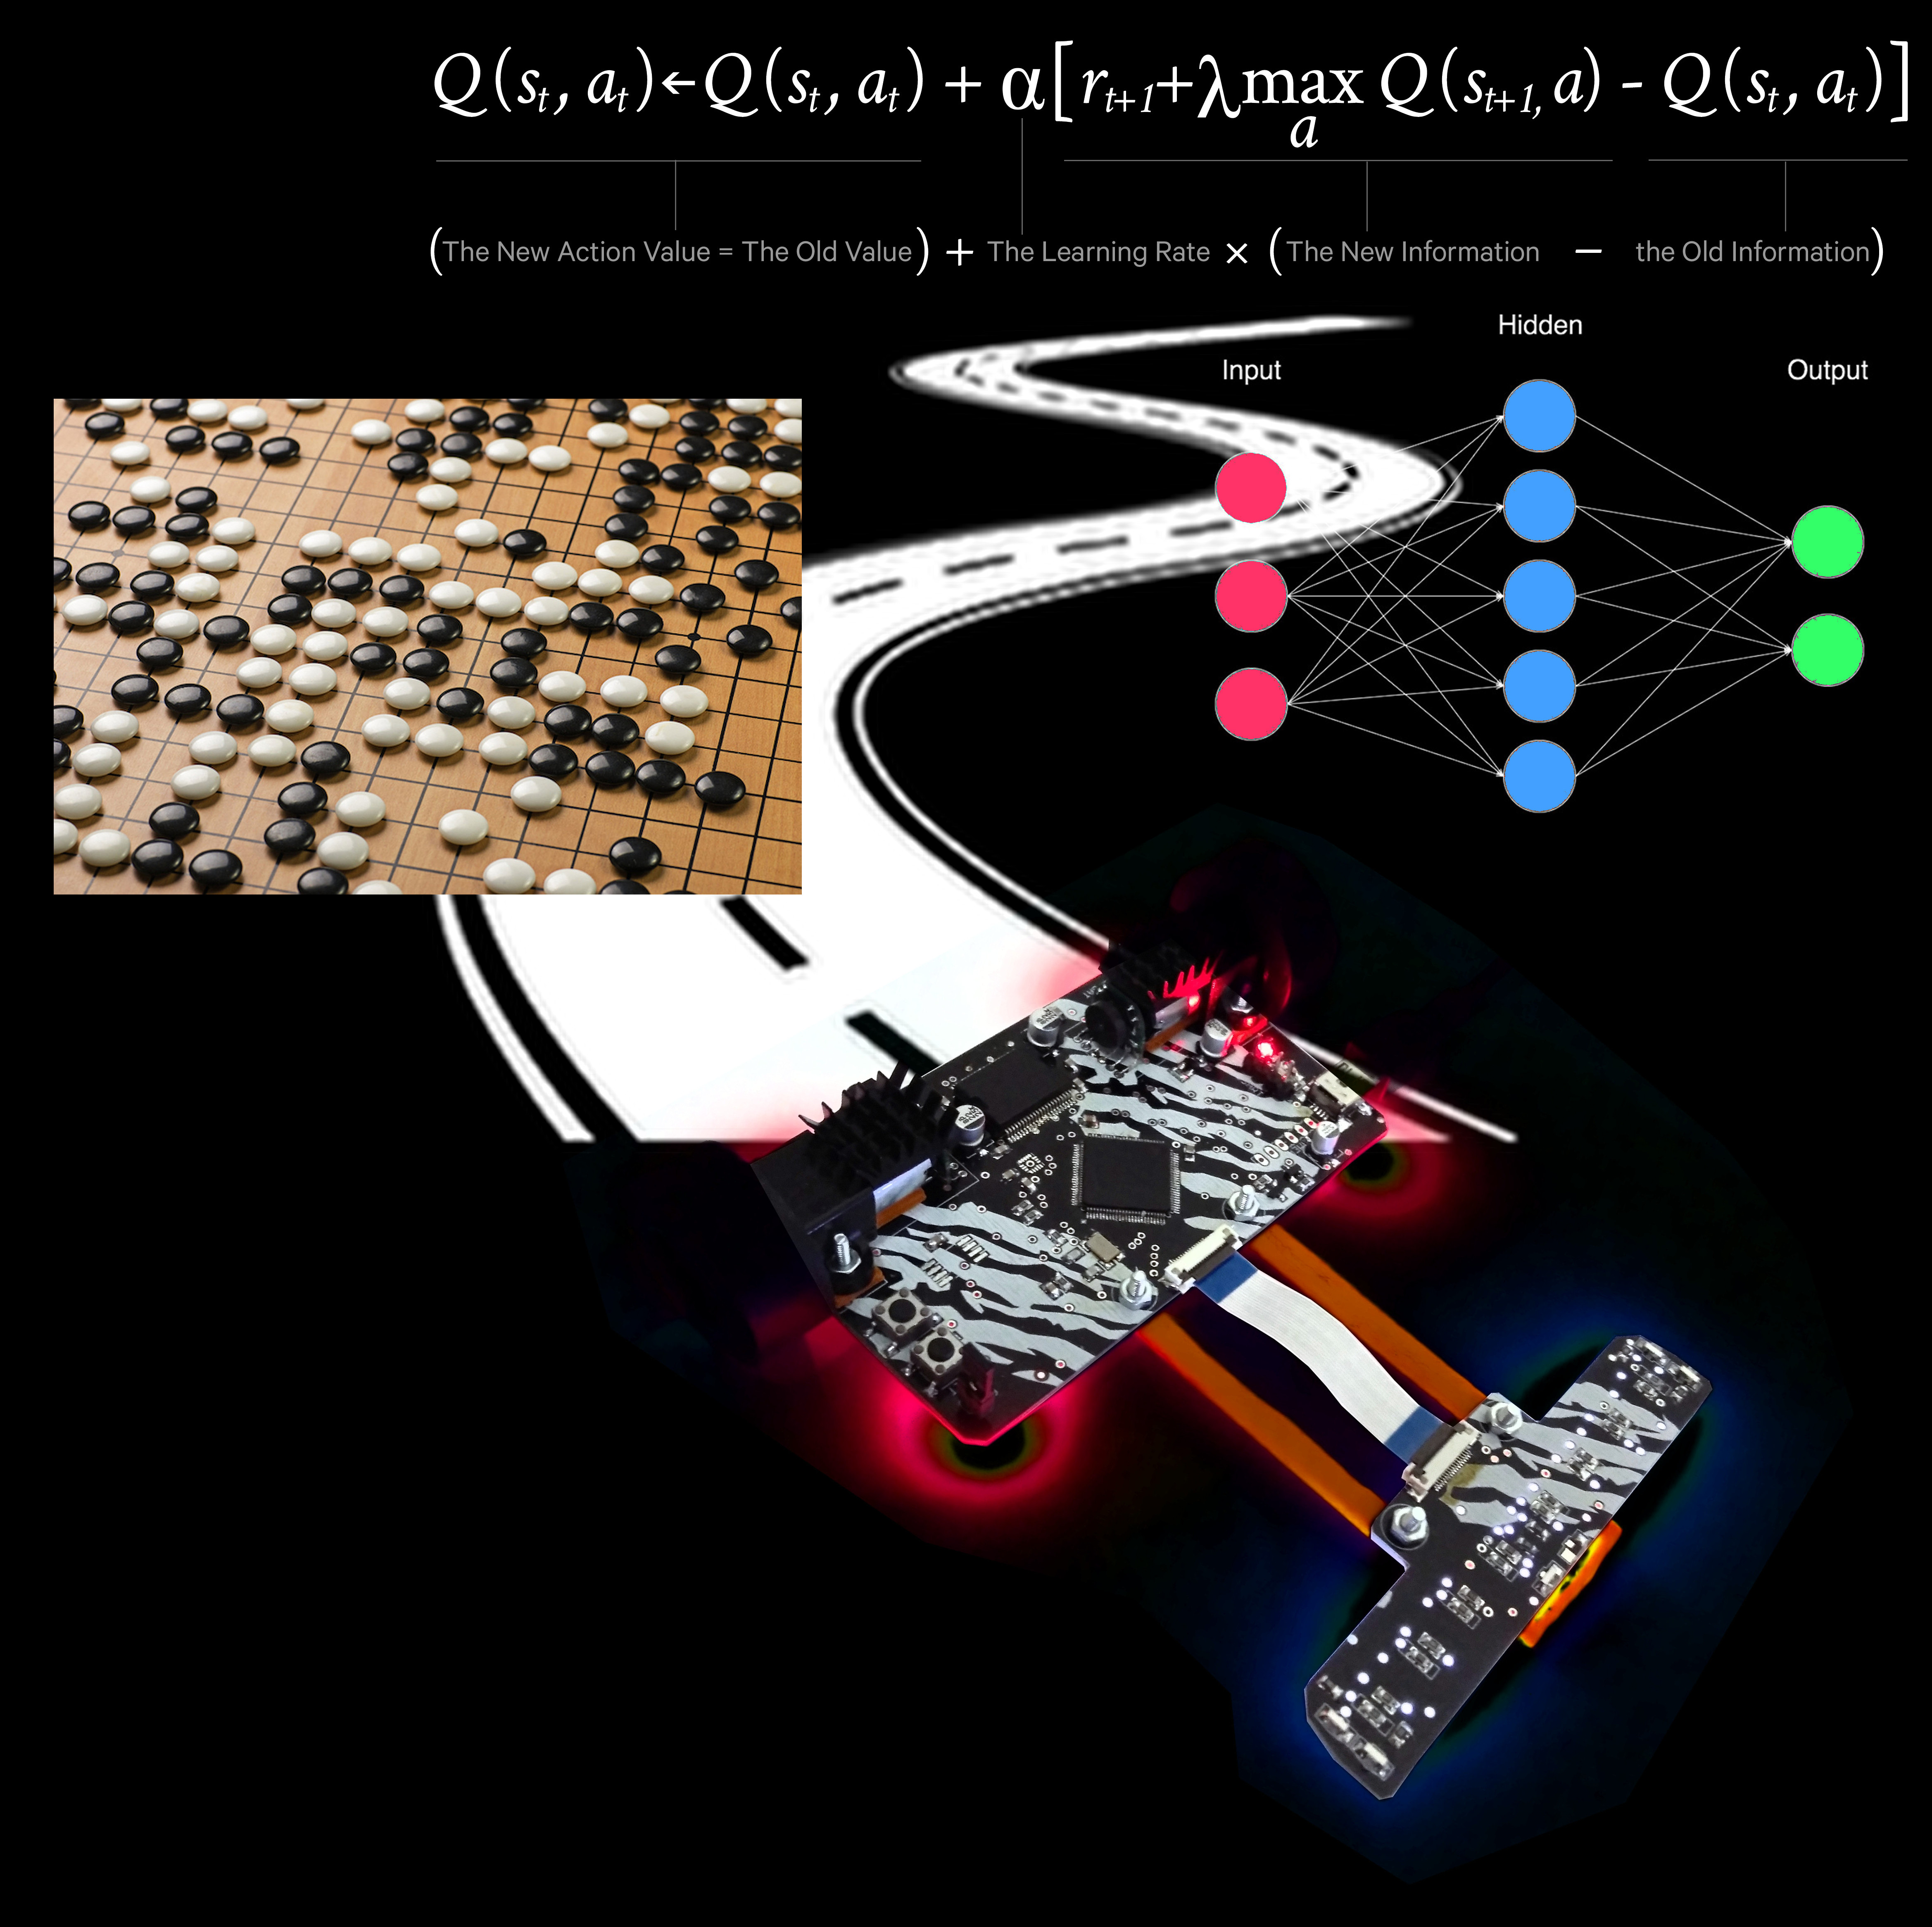
\includegraphics[width=5.05in]{./pictures/rl_square.jpg}}

        \hfil}\vfil}
    }
    \begin{frame}

    %\titlepage


    \centering
     \colorbox{black}
     {
        \begin{minipage}{7cm}
           {\LARGE \color{white} \bf training universal Atari gambler using \\ reinforcement learning} \\
           {\LARGE \color{white} Michal CHOVANEC} \\
       \end{minipage}
     }


    \end{frame}
}

\begin{frame}{\bf Reinforcement learning}
- learning from punishments and rewards


\begin{columns}
\begin{column}{0.5\textwidth}

    \centering
    \includemovie[
      poster,
      autoplay,
      externalviewer,
      inline=false,
      text={ 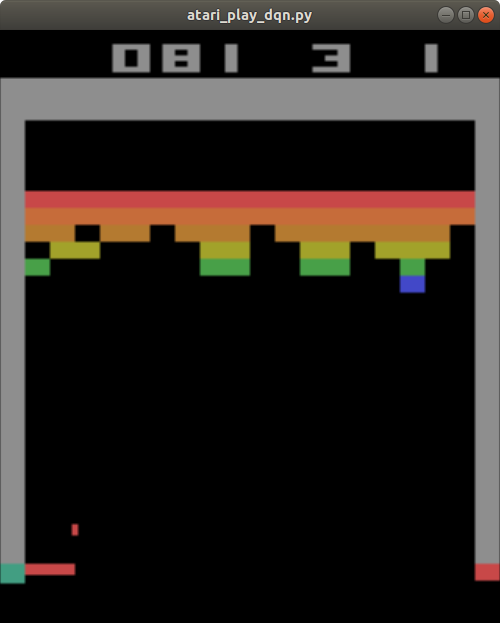
\includegraphics[scale=0.15]{./pictures/breakout.png}}
    ]{4cm}{4cm}{./video/rl_atari.mp4}

\begin{figure}
  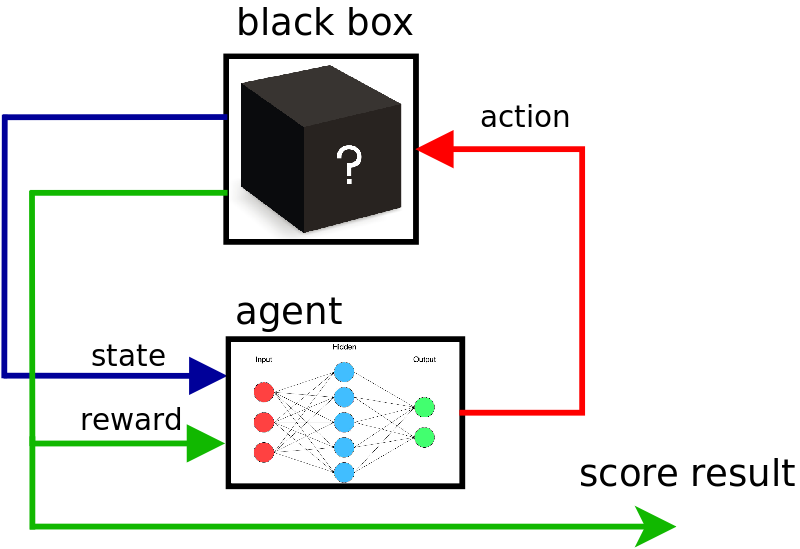
\includegraphics[scale=0.2]{./diagrams/rl_mechanism.png}
\end{figure}

\end{column}
\begin{column}{0.5\textwidth}  %%<--- here

\begin{itemize}
  \item obtain {\bf state}
  \item choose {\bf action}
  \item {\bf execute} action
  \item obtain {\bf reward}
  \item learn from {\bf experiences}, $Q(s, a)$, or $\pi(a|s)$
\end{itemize}


\end{column}
\end{columns}

\end{frame}


\begin{frame}{\bf deep Q network - DQN}

$Q(s, a)$ : what is the potential reward in state $s$ and action $a$

\begin{figure}
  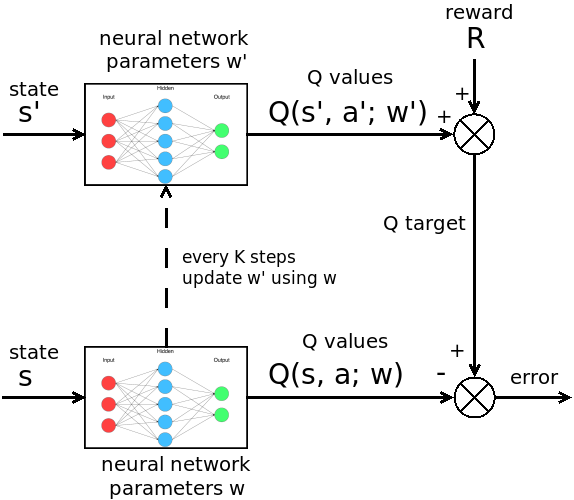
\includegraphics[scale=0.3]{./diagrams/dqn_detail.png}
\end{figure}

\begin{align*}
\mathcal{L}= &\left( \underset{\bf \color{green} target\ value}{ R + \gamma \max \limits_{\alpha'} Q(s', \alpha'; w') } - \underset{\bf \color{red} predicted\ value}{Q(s, a; w)} \right) ^2
\end{align*}

\end{frame}


\begin{frame}{\bf be more specific}
\begin{itemize}
  \item state  : \begin{itemize}
                  \item  grayscale frames, 
                  \item size 96x96, (84x84) 4 past frames - frame stacking
                  \item use wrappers (life lost reward, frame skipping, reset fire button)
                \end{itemize}
  \item reward : clip into range $\langle -1, 1 \rangle$
  \item discount factor $\gamma = 0.99$
  \item update rate $k = 4$
\end{itemize}


\begin{figure}
  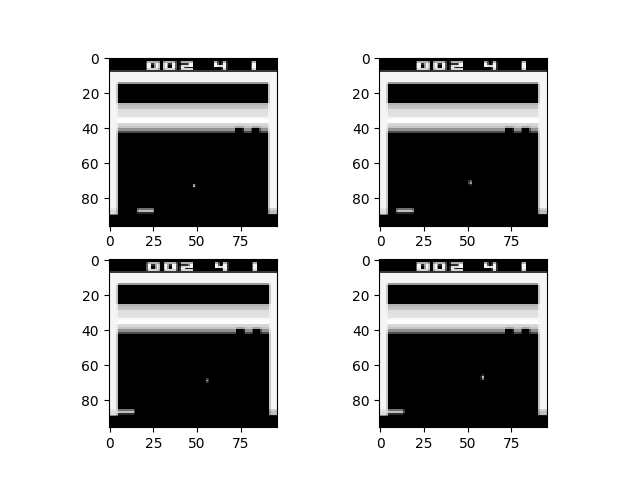
\includegraphics[scale=0.4]{./pictures/breakout_state.png}
\end{figure}

\end{frame}


\begin{frame}{\bf neural network architecture}
a long time ago in a galaxy far far away
\begin{itemize}
\item 2012 : Krizhevsky AlexNet : {\bf 11x11, 5x5, 3x3 kernels}   \footnote{\href{https://papers.nips.cc/paper/4824-imagenet-classification-with-deep-convolutional-neural-networks.pdf}{https://papers.nips.cc/paper/4824-imagenet-classification-with-deep-convolutional-neural-networks.pdf}}
\item 2013 : Playing Atari with Deep Reinforcement Learning, Mnih et. al. : {\bf 8x8, 4x4 kernels} Krizhevsky framework \footnote{\href{https://arxiv.org/abs/1312.5602}{https://arxiv.org/abs/1312.5602}}
\end{itemize}

\begin{figure}
  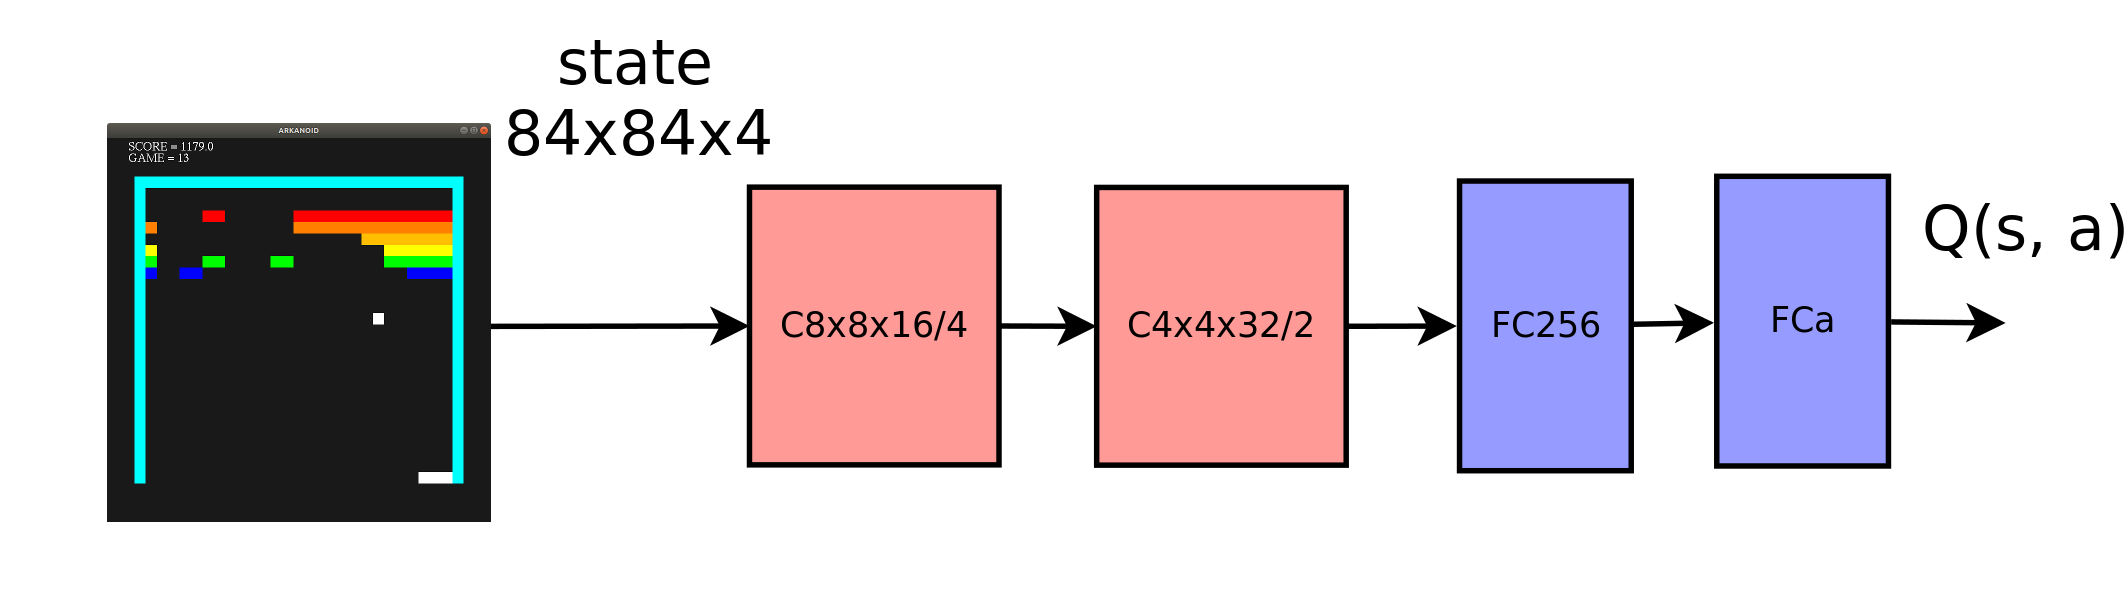
\includegraphics[scale=0.18]{./diagrams/dqn_mnih_atari.png}
\end{figure}

\end{frame}


\begin{frame}{\bf neural network architecture}


\begin{itemize}
\item state 96x96, $3*2^5$ - allows deeper architecture
\item only 3x3 kernels, less computations costs
\item deeper architecture
\item compare with recent MuZero paper - Mastering Atari, Go, Chess and Shogi by Planning with a Learned Model \footnote{\href{https://arxiv.org/abs/1911.08265}{https://arxiv.org/abs/1911.08265}}
\end{itemize}

\begin{figure}
  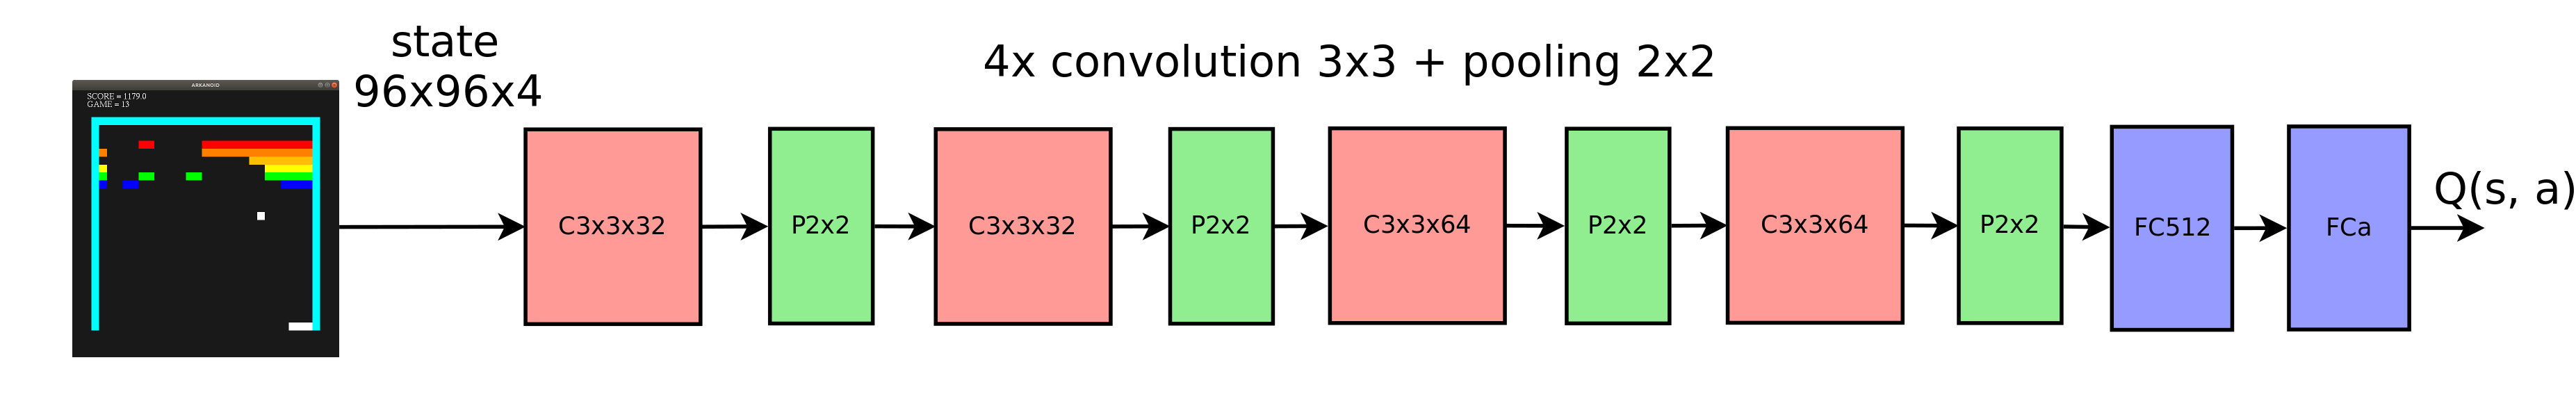
\includegraphics[scale=0.11]{./diagrams/dqn_my_atari.png}
\end{figure}

\end{frame}


\begin{frame}{\bf neural network architecture}
\begin{figure}
  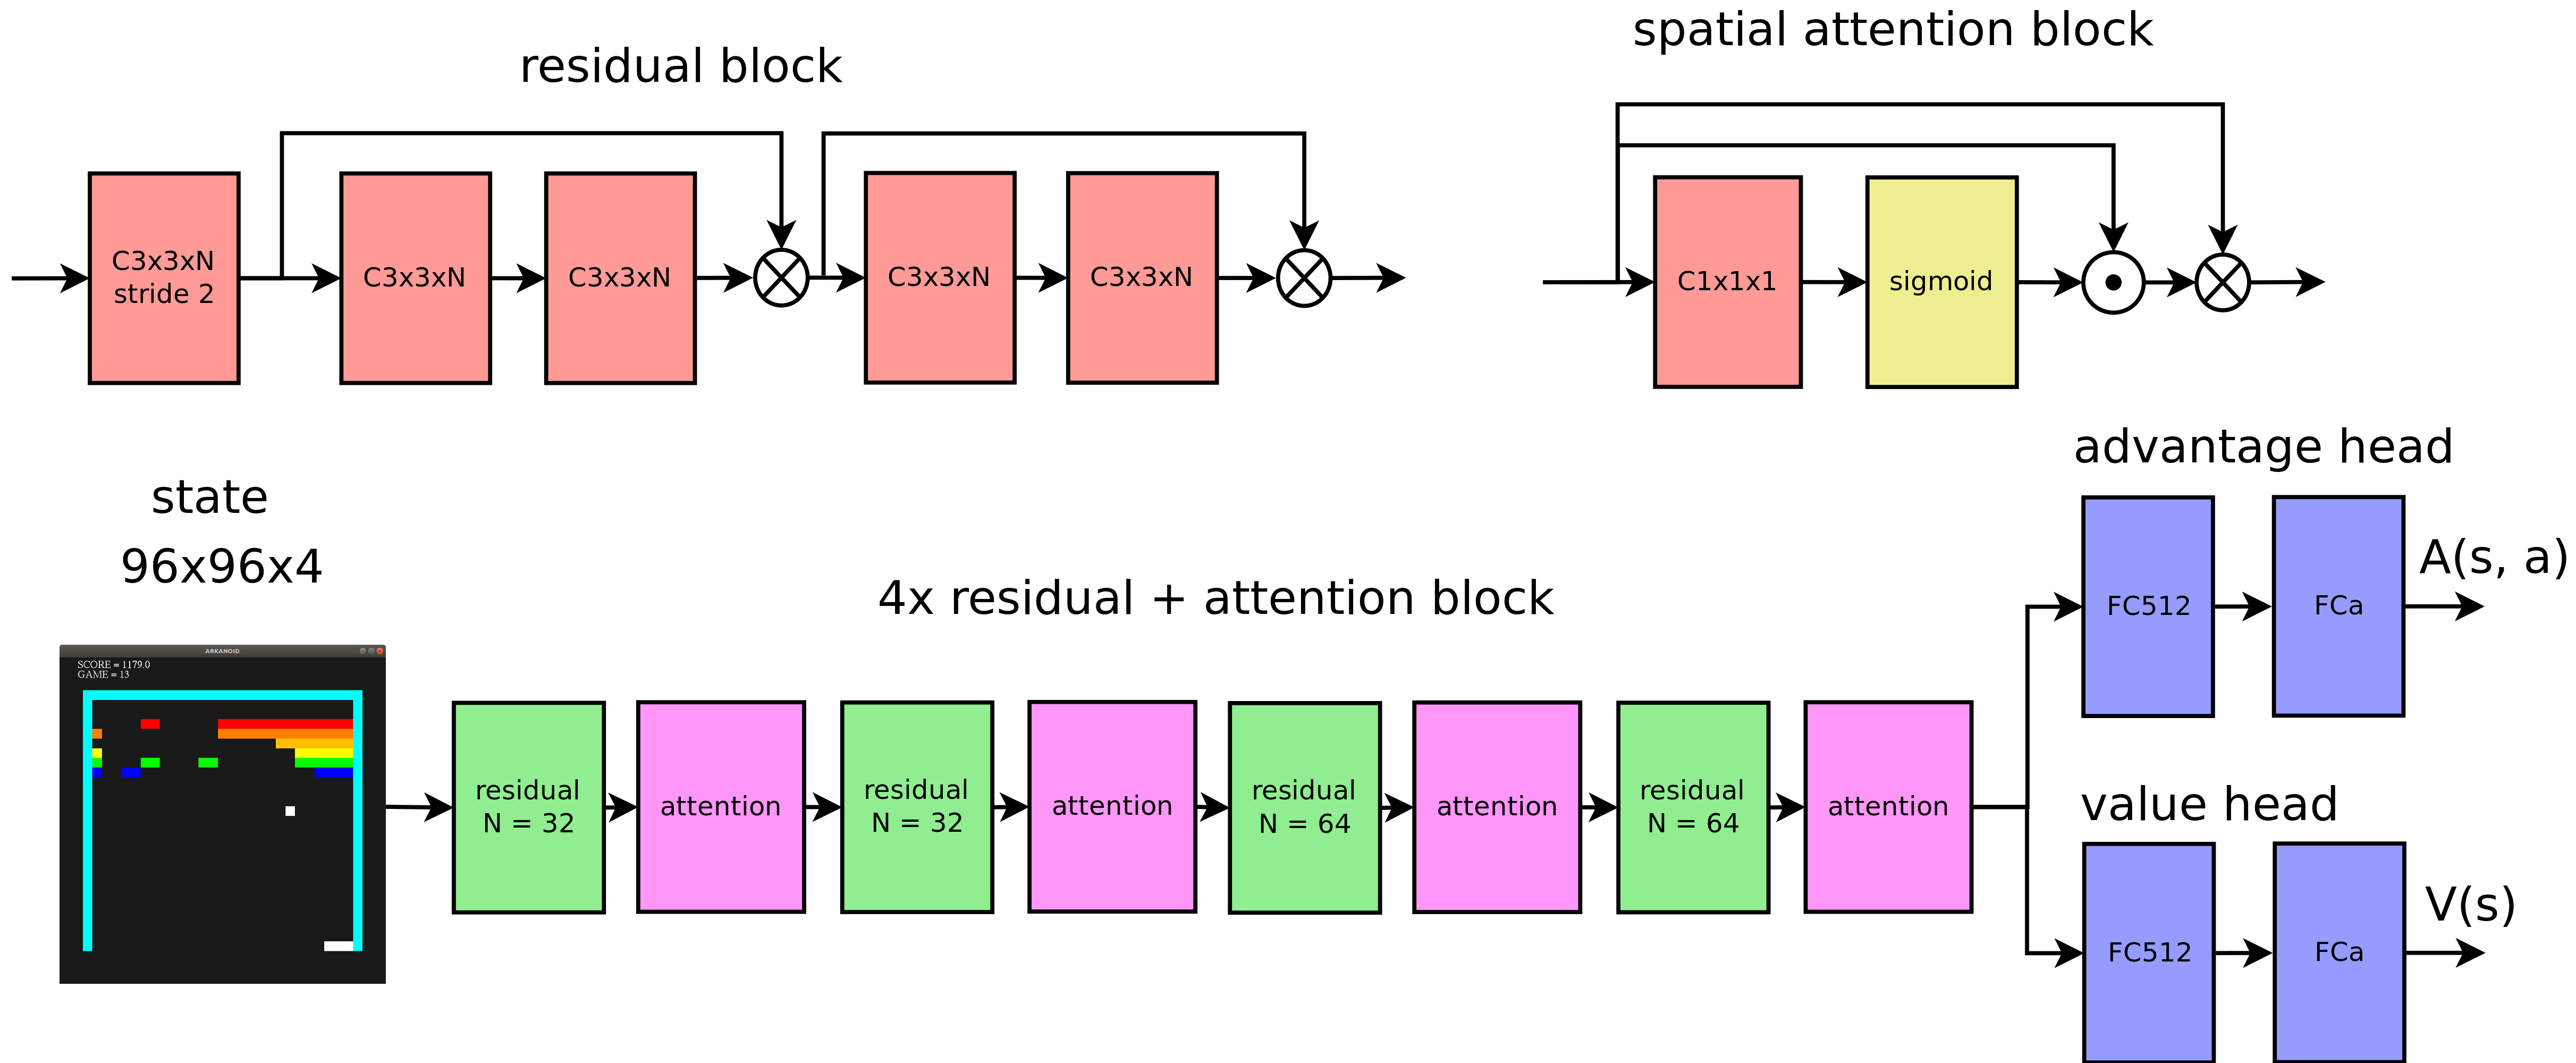
\includegraphics[scale=0.08]{./diagrams/attention_dueling_dqn_my_atari.png}
\end{figure}
\end{frame}


\begin{frame}{\bf playing multiple games using one network}


\begin{columns}

  \begin{column}{0.25\textwidth}
    \begin{figure}
      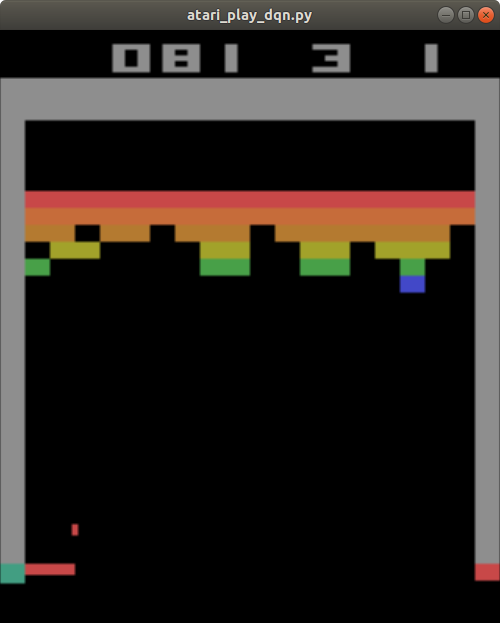
\includegraphics[scale=0.15]{./pictures/breakout.png}
    \end{figure}
  \end{column}

  \begin{column}{0.25\textwidth}
    \begin{figure}
      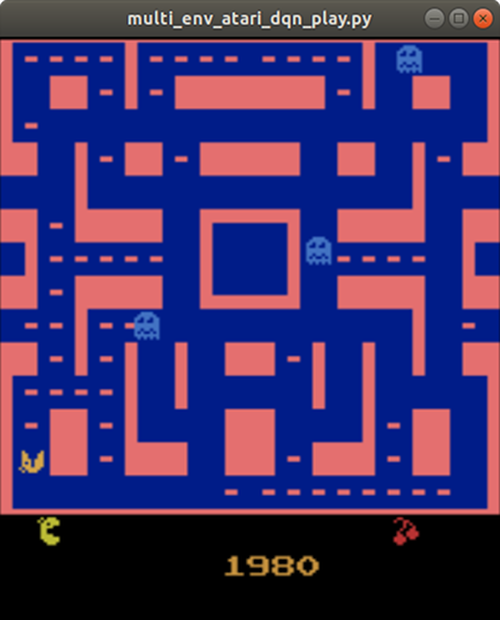
\includegraphics[scale=0.15]{./pictures/pacman.png}
    \end{figure}
  \end{column}

  \begin{column}{0.25\textwidth}
    \begin{figure}
      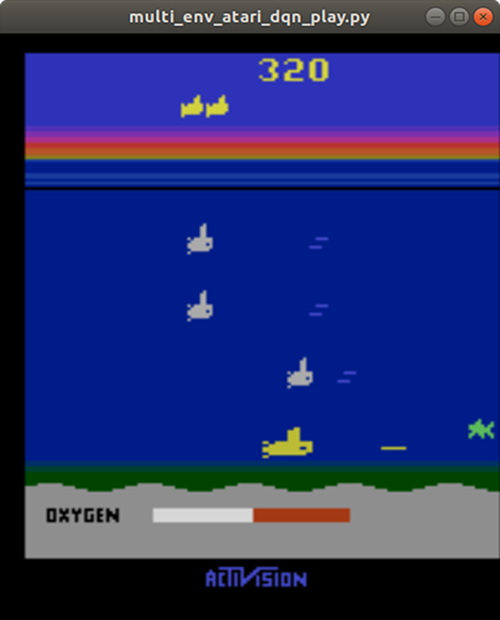
\includegraphics[scale=0.15]{./pictures/seaquest.png}
    \end{figure}
  \end{column}

  \begin{column}{0.25\textwidth}
    \begin{figure}
      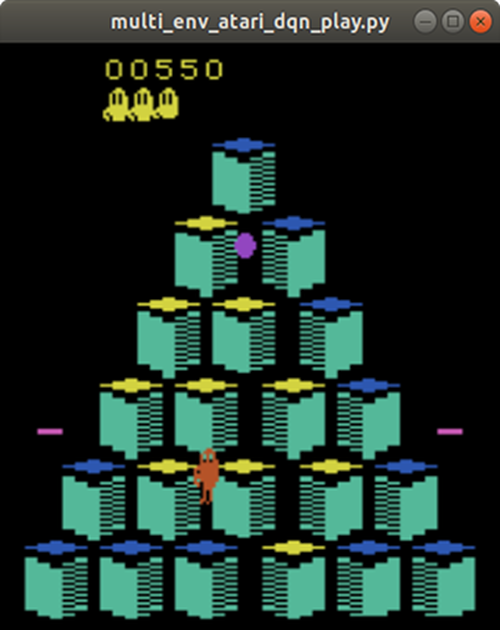
\includegraphics[scale=0.15]{./pictures/qbert.png}
    \end{figure}
  \end{column}


\end{columns}

\begin{itemize}
  \item pure DQN
  \item dueling residual DQN
  \item dueling residual DQN with attention
\end{itemize}




\end{frame}






\begin{frame}{\bf results : attention is all you need}

\begin{columns}

  \begin{column}{0.5\textwidth}
    \begin{figure}
      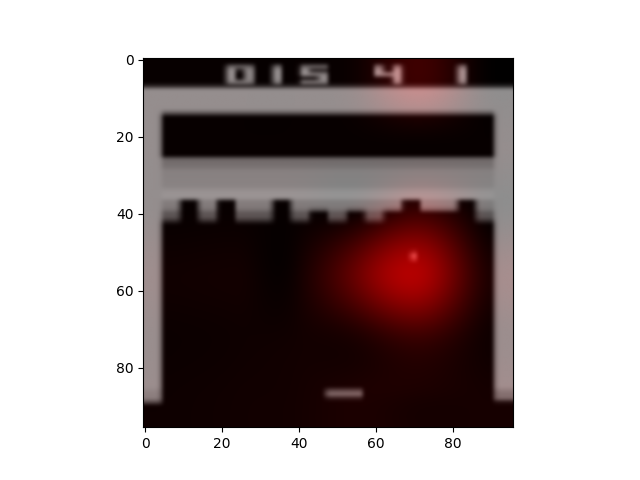
\includegraphics[scale=0.3]{./pictures/attention_breakout_dqn.png}
    \end{figure}
  \end{column}

  \begin{column}{0.5\textwidth}
    \begin{figure}
      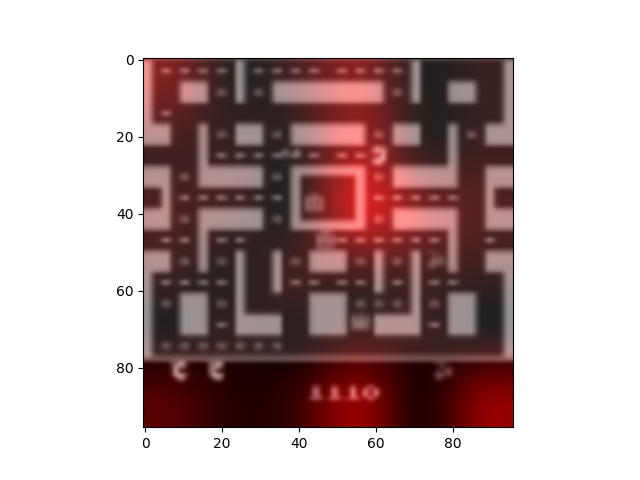
\includegraphics[scale=0.3]{./pictures/attention_pacman_dqn.png}
    \end{figure}
  \end{column}


\end{columns}

\begin{columns}

  \begin{column}{0.5\textwidth}
    \begin{figure}
      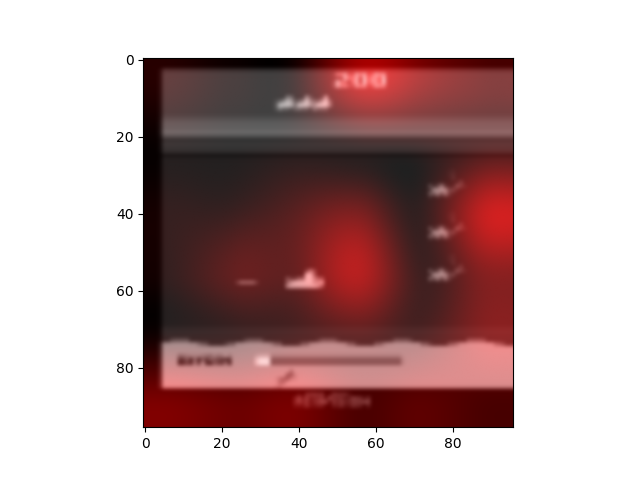
\includegraphics[scale=0.3]{./pictures/attention_seaquest_dqn.png}
    \end{figure}
  \end{column}

  \begin{column}{0.5\textwidth}
    \begin{figure}
      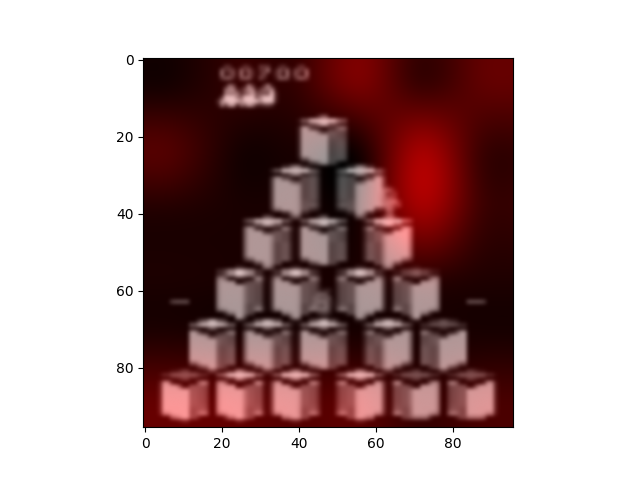
\includegraphics[scale=0.3]{./pictures/attention_qbert_dqn.png}
    \end{figure}
  \end{column}


\end{columns}

\end{frame}




\begin{frame}{\bf results : kernel response visualisation}

\begin{align*}
\mathcal{L}= -2\overline{y_{lk}(x)} + \overline{y(x)}
\end{align*}

    \begin{figure}
      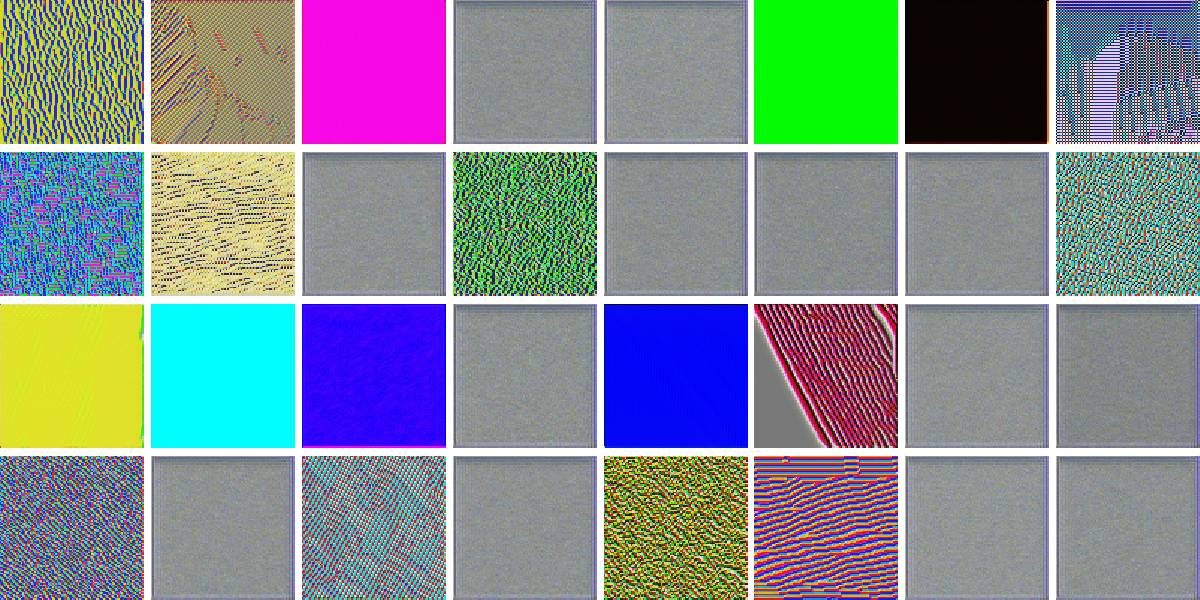
\includegraphics[scale=0.3]{./pictures/kernel_visualisation/0.png}
    \end{figure}

    \begin{figure}
      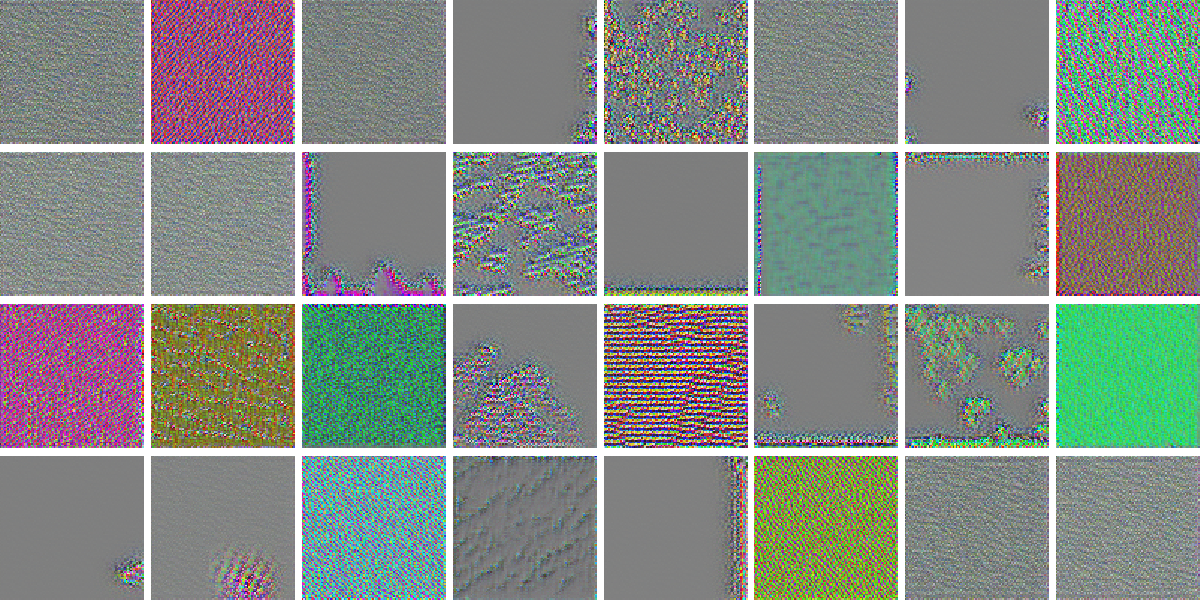
\includegraphics[scale=0.3]{./pictures/kernel_visualisation/3.png}
    \end{figure}


\end{frame}


\begin{frame}{\bf results : kernel response visualisation}

\begin{align*}
\mathcal{L}= -2\overline{y_{lk}(x)} + \overline{y(x)}
\end{align*}

    \begin{figure}
      
\includegraphics[scale=0.3]{./pictures/kernel_visualisation/6.png}
    \end{figure}




\end{frame}




\begin{frame}{\bf results : farewell my dear gtx1080ti}
\begin{figure}
  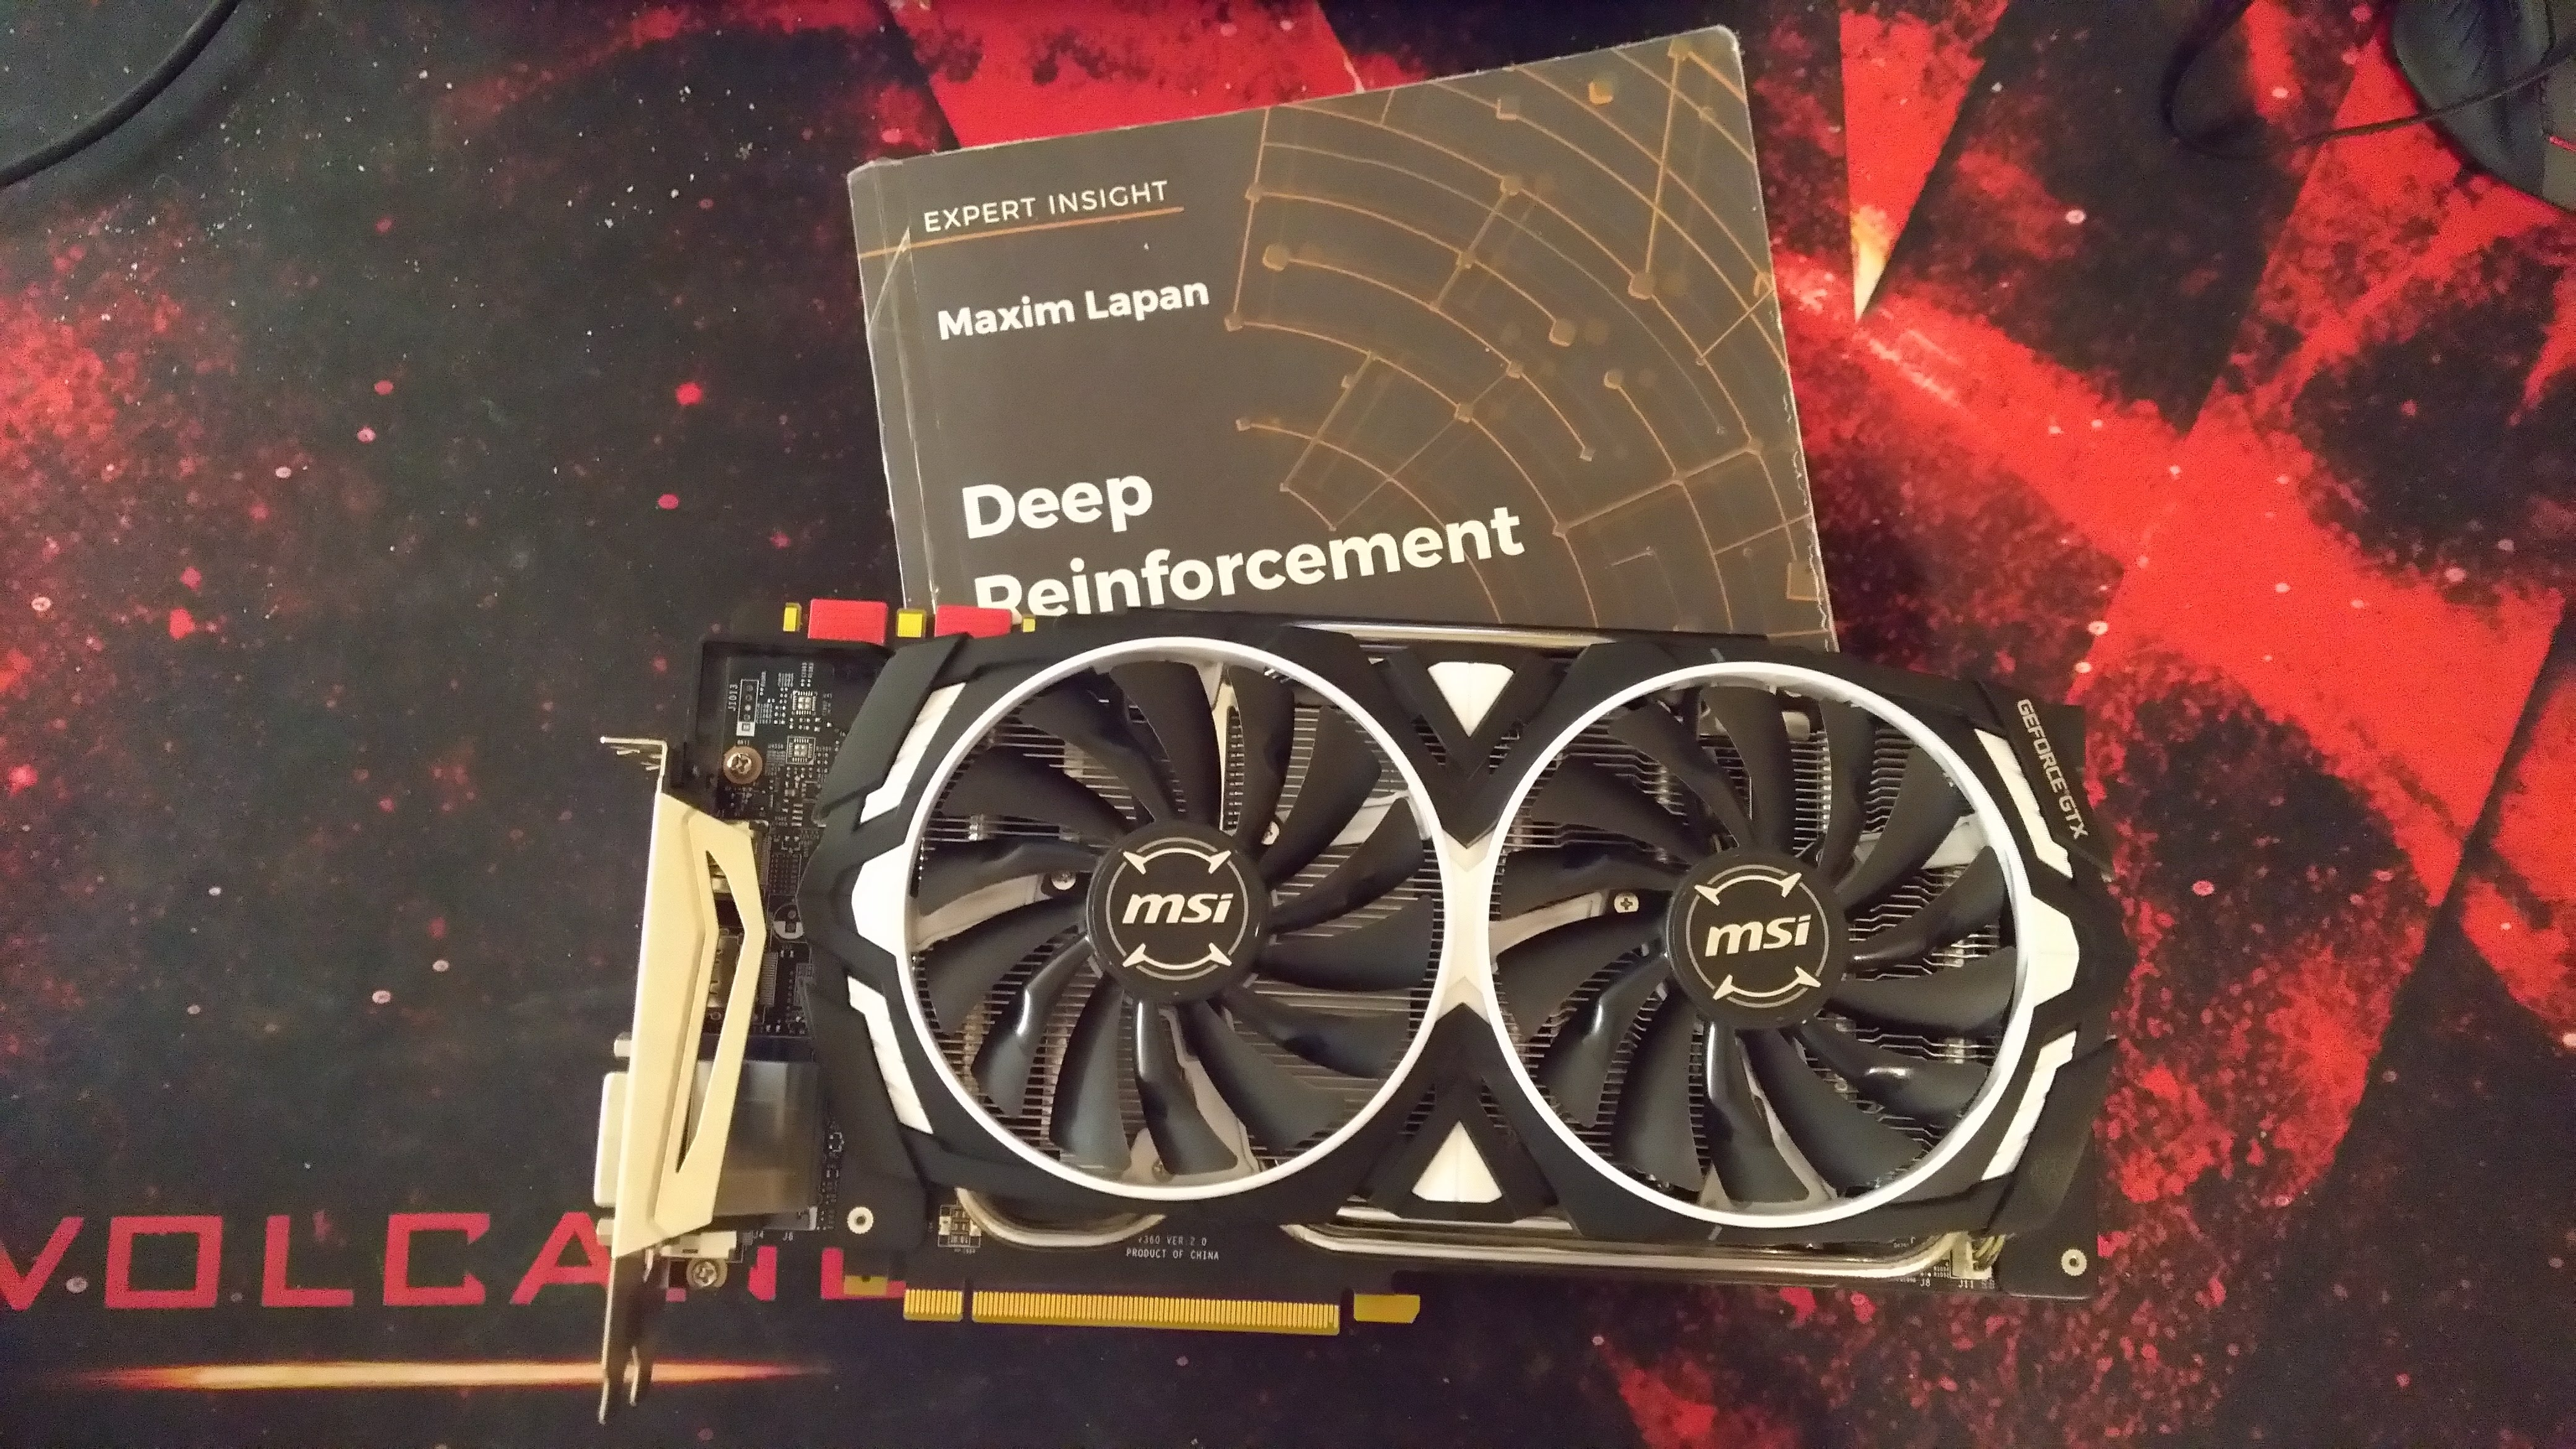
\includegraphics[scale=0.08]{./pictures/gtx1080ti.jpg}
\end{figure}
\end{frame}



\begin{frame}{\bf RL magic chart}
\setbeamercolor{background canvas}{bg=black}
There is no classification, no regression, no RL, there is only LOSS function

{\bf Value based methods}

DQN : 
\begin{align*}
\mathcal{L}= &\left( R + \gamma \max \limits_{\alpha'} Q(s', \alpha'; \theta ') - Q(s, a; \theta) \right) ^2
\end{align*}

Dueling DQN : 
{\small
\begin{align*}
\mathcal{L}= \left(  R + \gamma \max \limits_{\alpha'} Q(s', \alpha'; \theta ') - \left( V(s; \theta) + A(s, a; \theta) - \frac{1}{N}\sum_{\alpha} A(s, \alpha; \theta) \right) \right)^2
\end{align*}
}
\end{frame}






\begin{frame}{\bf RL magic chart}
There is no classification, no regression, no RL, there is only LOSS function

{\bf Policy based methods}

Reinforce : 
\begin{align*}
\mathcal{L}&= -V(n) log \pi(s(n), a(n); \theta) \\
       V(n)&= R(n) + \gamma V(n+1)
\end{align*}

Actor critic : 
\begin{align*}
\mathcal{L}_{actor}&= -Q(s; \phi) log \pi(s, a; \theta) \\
\mathcal{L}_{critic}&= \left( R(n) + \gamma Q(s(n+1); \phi) - Q(s(n); \phi)  \right)^2
\end{align*}

Advantage actor critic : 
\begin{align*}
\mathcal{L}_{actor}&= -\left( R(n) + \gamma Q(s(n+1); \phi) - Q(s(n); \phi)  \right) log \pi(s, a; \theta) \\
\mathcal{L}_{critic}&= \left( R(n) + \gamma Q(s(n+1); \phi) - Q(s(n); \phi)  \right)^2 \\
\mathcal{L}_{entropy}&= - \sum_a \pi(s, a; \theta) log \pi(s, a; \theta)
\end{align*}

\end{frame}



\begin{frame}{\bf Q\&A - consultations on Rysy Hut 2250 m.a.s.l.}
 \vspace{-6mm}
\begin{figure}
  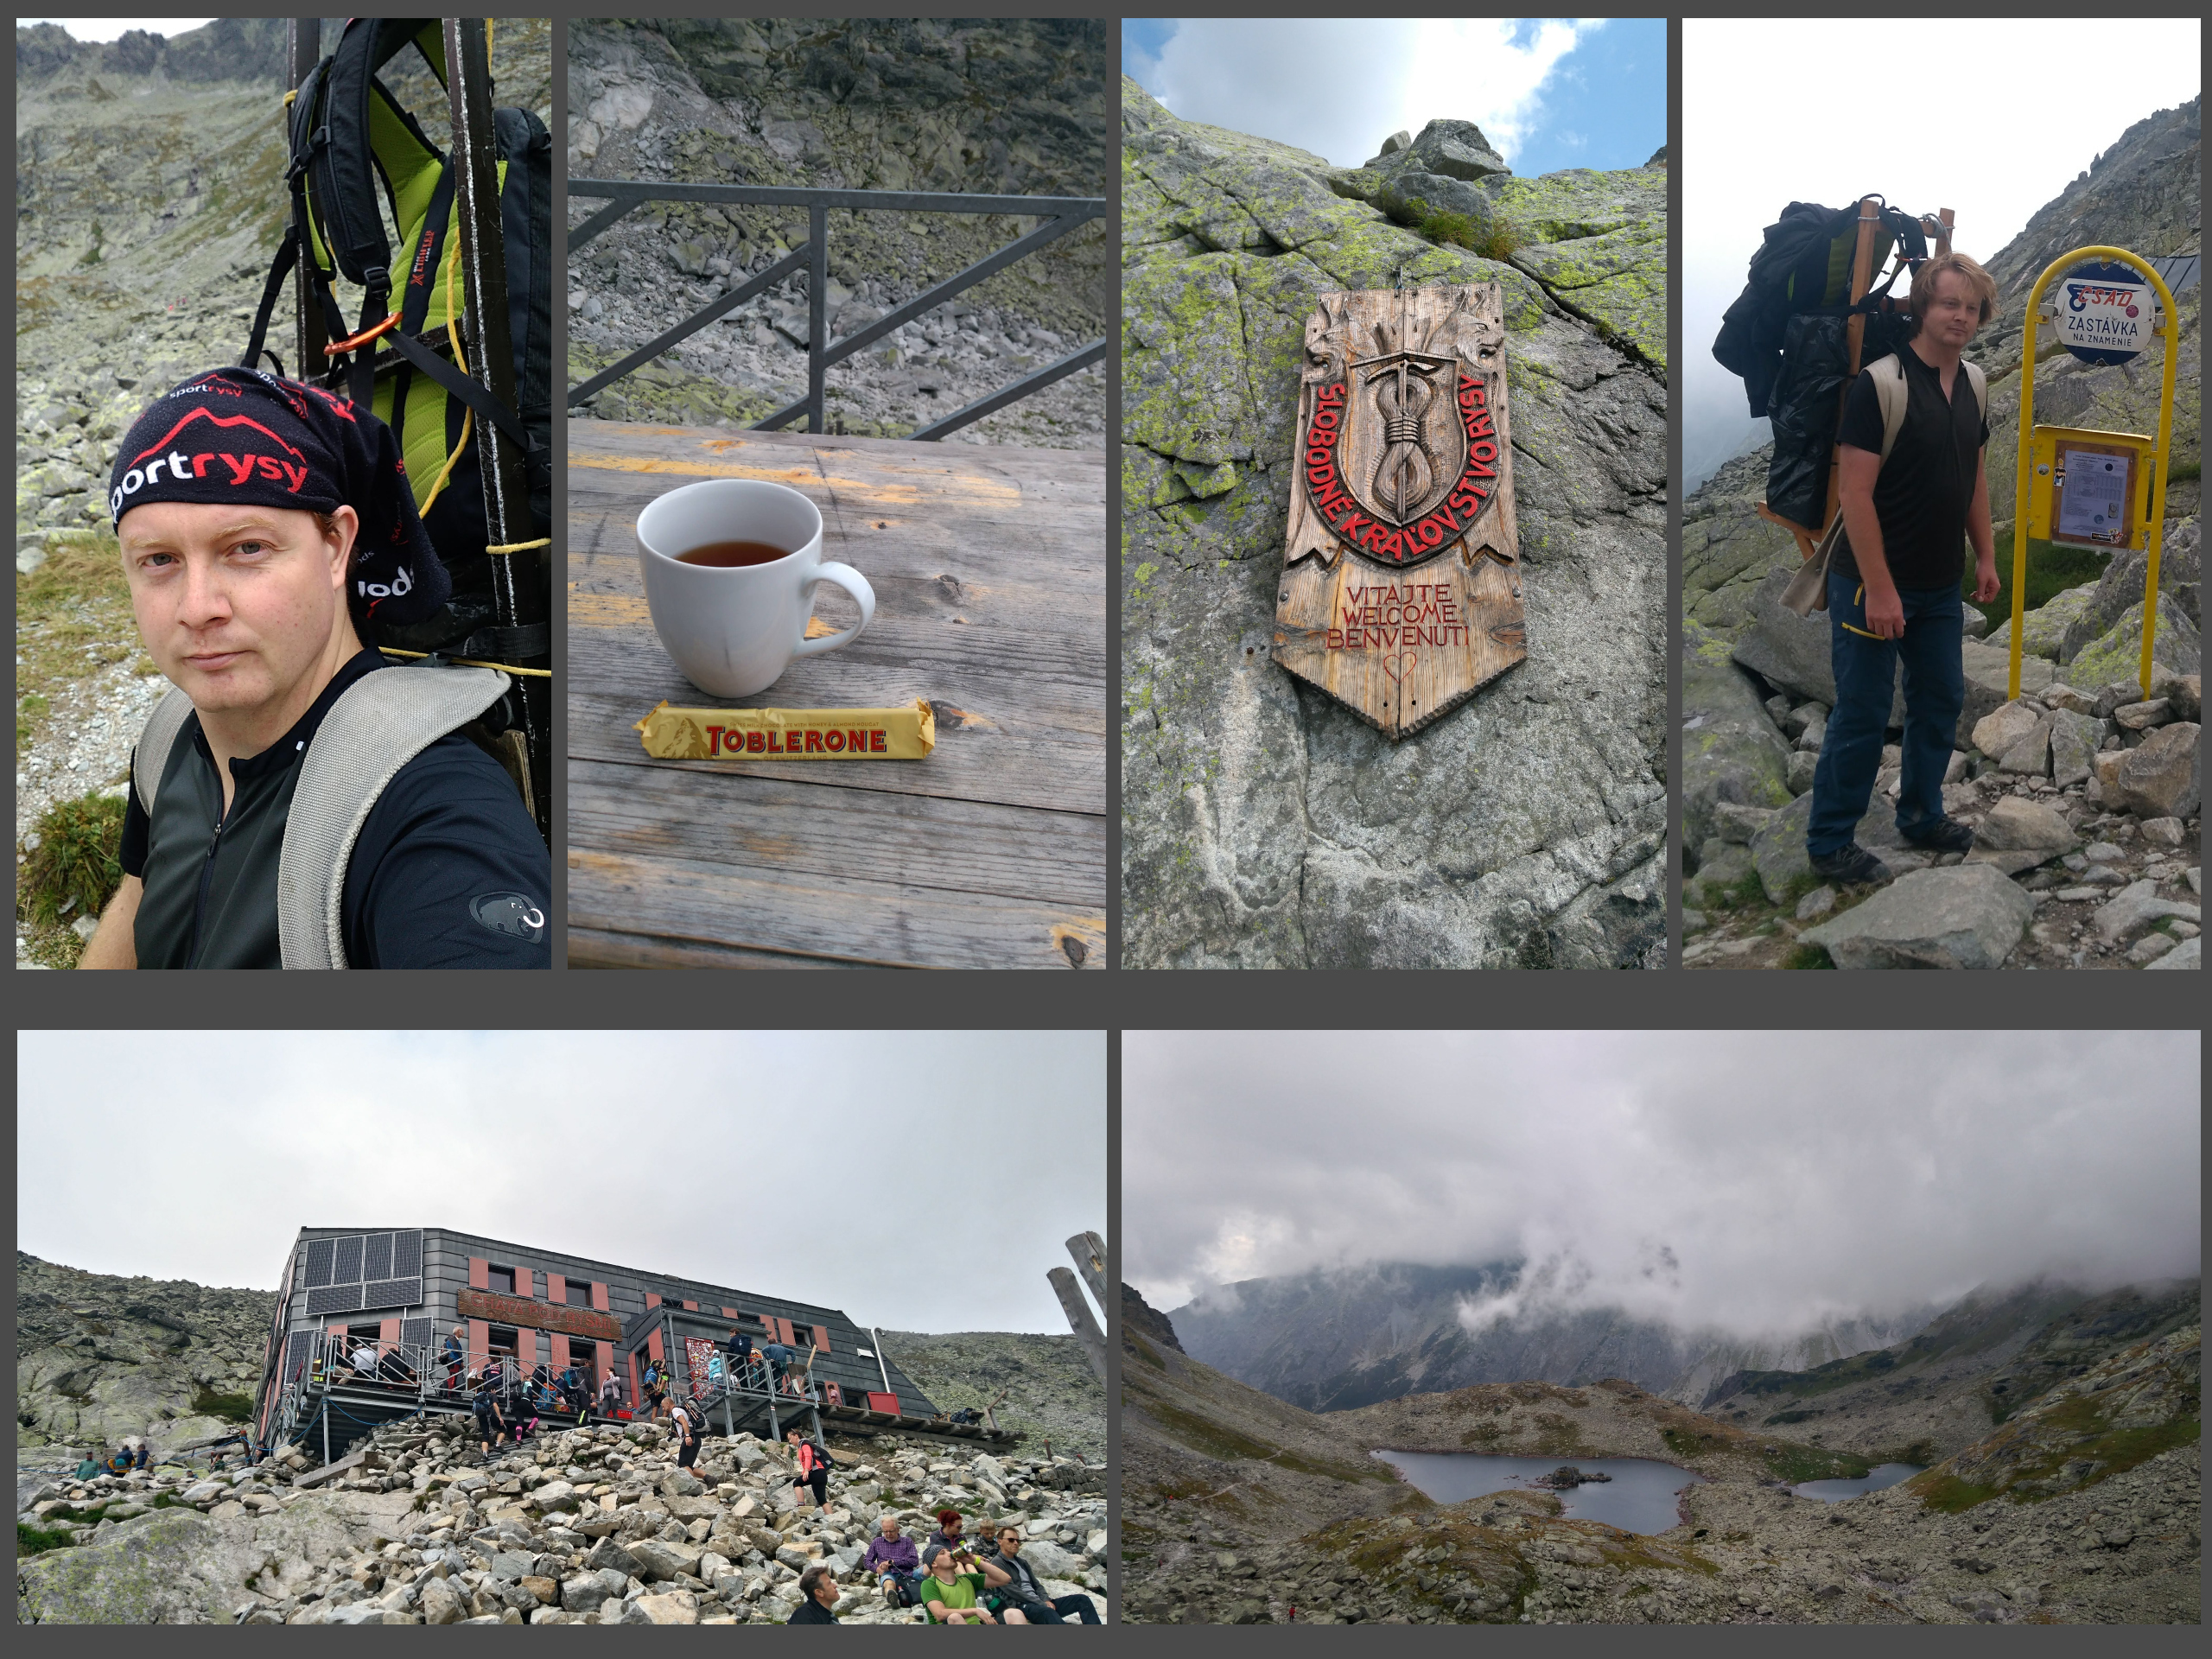
\includegraphics[scale=0.5]{./pictures/me_rysy.jpg}
\end{figure}

\end{frame}


\end{document}
